% This file was created with tikzplotlib v0.10.1.
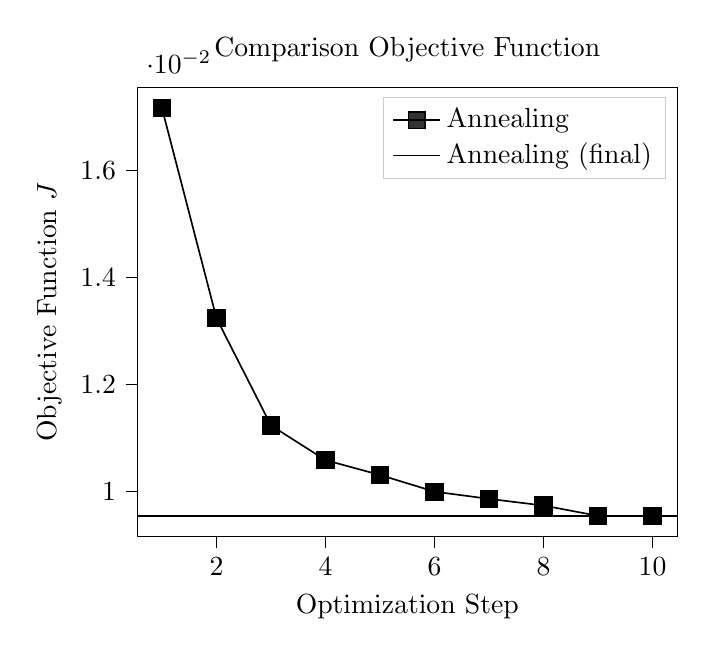
\begin{tikzpicture}

\definecolor{darkgray176}{RGB}{176,176,176}
\definecolor{lightgray204}{RGB}{204,204,204}

\begin{axis}[
legend cell align={left},
legend style={fill opacity=0.8, draw opacity=1, text opacity=1, draw=lightgray204},
tick align=outside,
tick pos=left,
title={Comparison Objective Function},
x grid style={darkgray176},
xlabel={Optimization Step},
xmin=0.55, xmax=10.45,
xtick style={color=black},
y grid style={darkgray176},
ylabel={Objective Function \(\displaystyle J\)},
ymin=0.00916897120744358, ymax=0.0175368835036707,
ytick style={color=black}
]
\addplot [semithick, black, mark=square*, mark size=3, mark options={solid}]
table {%
1 0.0171565238538422
2 0.0132377311120647
3 0.0112367086861626
4 0.0105889811007124
5 0.0103121631866096
6 0.0100009806128386
7 0.00986610247593014
8 0.00974160302562563
9 0.00954933085727208
10 0.00954933085727208
};
\addlegendentry{Annealing}
\addplot [semithick, black]
table {%
0.55 0.00954933085727208
10.45 0.00954933085727208
};
\addlegendentry{Annealing (final)}
\end{axis}

\end{tikzpicture}
